%%=========================
%% Section 1.02: Origins of the Green's Functions and Roots of P
%%=========================

\documentclass[../dissertation.tex]{subfiles}

\begin{document}
\section{Motivation of the Green's Functions}\label{sec1:RootsOfP}

To motivate our choice of Green's function for this linear spectral
problem, suppose there exists a function $G$ satisfying 
$L_\delta(G^+)(x) = \delta_0(x)$, 
where $\delta_0(x)$\label{sym:dirac} denotes the Dirac delta function (not to be confused with 
the parameter $\delta$). Formally, by taking the Fourier 
transform\label{sym:fourier} of both 
sides of $L_\delta(G^+)(x) = \delta_0(x)$, we have
\[
	1 
		= \xi \, \wh G^+ - \zeta \( \wh G^+ - \wh G^- \)
		= \big[ \xi - \zeta \(1 - e^{-2\delta\xi}\) \big] \wh G^+
		= p(\xi; \zeta, \delta) \, \wh G^+,
\]
where 
\begin{align*}
	p(\xi; \lambda, \delta) 
		&= \xi - \zeta\(1 - e^{-2\delta \xi}\) \\
		&= \( \frac{\xi}{1 - e^{-2\delta \xi}} - \zeta \)\(1 - e^{-2\delta \xi}\) \\
		&= \big(\zeta(\xi) - \zeta(\lambda)\big)\(1 - e^{-2\delta \xi}\).
\end{align*}
However, this approach is somewhat problematic, given that the function $p$ has 
roots $\xi = 0$ and $\xi = \lambda$ along the real line. So, instead defining 
a single Green's function for the spectral problem \eqref{eq:JostDE} based on 
taking the inverse Fourier transform of $1/p$, we instead define two different 
Green's functions $G_L^+$ and $G_R^+$ based on taking two different ``Fourier 
inverse like'' transforms of $1/p$ for which the respective contours of 
integration avoids the roots of $p$. Specifically, 
	\begin{align*}
		G_L^+(x; \lambda, \delta)
			&:= 
				\frac{1}{2\pi} 
				\int_{\Gamma_L} 
					e^{i\xi x} \frac{1}{p(\xi; \lambda, \delta)} \, 
				d\xi \\
		G_R^+(x; \lambda, \delta) 
			&:= 
				\frac{1}{2\pi} 
				\int_{\Gamma_R} 
					e^{i\xi x} \frac{1}{p(\xi; \lambda, \delta)} 
				\, \mathrm{d}\xi
	\end{align*}
where the contour ${\Gamma_L}$ bypasses the roots $\xi = 0$ and $\xi = \lambda$ 
from below, and the contour ${\Gamma_R}$ bypasses the roots $\xi = 0$ and 
$\xi = \lambda$ from above, as mentioned in the previous section. 


Since $p(\xi; \lambda)$ can be rewritten as
\[
	p(\xi; \lambda) 
		= \(\frac{\xi}{1-e^{-2 \xi \delta}}-\zeta(\lambda)\)\(1-e^{-2 \xi \delta}\)
		= \big( \zeta(\xi) - \zeta(\lambda) \big)\(1 - e^{-2\xi \delta}\),
\]
it is easy to check that both $\xi = 0$ and $\xi = \lambda$ are roots of $p$. 
In the remainder of this section, we argue that these are the only roots of 
$p$ in the strip
\[
	\mathcal R_\delta:= \left\{z\in\CC ~:~ -\frac{\pi}{\delta}\leq\im z\leq\frac{\pi}{\delta} \right\}
\]
as is defined in the Introduction of this chapter.
That is, we show that the equation
\begin{align} \label{eq1:baseEqn}
	\xi - \zeta(\lambda) + \zeta(\lambda) e^{-2 \xi \delta} = 0
\end{align}
has exactly two solutions (in $\xi$) for $\xi \in \mc R_\delta$. With a little algebraic 
manipulation, equation \eqref{eq1:baseEqn} can be rewritten as 
\begin{align} \label{eq1:EqnToSolve}
	\big(2 \delta \xi - 2 \delta \, \zeta(\lambda)\big) \, e^{2 \delta \xi - 2 \delta \, \zeta(\lambda)} 
		= -2 \delta \, \zeta(\lambda) \, e^{-2 \delta \, \zeta(\lambda)}.
\end{align}
In order to ``solve'' \eqref{eq1:EqnToSolve}, recall that the Lambert $W$ function 
(which we henceforth refer to only as $W$) is defined to be the multivalued 
``inverse'' of the function $z e^z$. So, to determine the number
of solutions \eqref{eq1:EqnToSolve} has for $\xi \in \mc R_\delta$, we need to specify 
which branches of $W$ are appropriate to apply to both sides of \eqref{eq1:EqnToSolve} 
given our restriction on $\xi$. 

The following discussion of the branches of the complex $W$\label{sym1:Wk} function is heavily 
inspired by Section 4 from the 1996 R.M. Corless, G.H. Gonnet, D.E.G. Hare, D.J. 
Jeffery and D.E. Knuth paper \cite{Corless1996}. As is the case with the standard 
complex exponential 
and logarithmic functions, to define the branches of $W$, the canonical approach 
is to make a branch cut along the negative real axis of the range of $z e^z$, and 
determine which curves in the range of $W$ are mapped to the branch cut ({\em i.e.} 
the negative real axis).

To do so, set 
\[
	\begin{aligned}
		z &:= w e^w  & \qquad w&:= W(z) \\
		  &:= x + i y & \qquad &:= t + i s.
	\end{aligned}
\]
Then, using Euler's formula to simply the equation
\[
	( x + i y) = (t + i s) e^{t + i s}
\]
and taking real and imaginary parts, we obtain the system
\[
	\left\{
		\begin{aligned}
			x&= e^t \(t \cos s - s \sin s\) \\
			y&= e^t \( t \sin s + s \cos s \).
		\end{aligned}
	\right.
\]
So, if $y=0$, then either $s = 0$ or $t = - s \cot s$. Further, $x < 0$ if and 
only if $t \cos s - s \sin s < 0$. Now, since $t = - s \cot s$ has asymptotes at 
$s = k \pi$ ($k \in \ZZ \sm \{0\}$), and the function $t \cos s - s \sin s$ has 
no roots, the inequality $t \cos s - s \sin s < 0$ holds precisely on the intervals
\[
	\(\bigcup_{-k \in \NN} \big( (2k + 1) \pi, \, 2 k \pi\big)\)
		\cup (-\pi, \,  \pi) \cup
		\( \bigcup_{k \in \NN} \big(2 k \pi, \,  (2k + 1) \)
\]
As such, the only curves the function $z e^z$ maps to the negative real axis are 
\[
	\gamma_k(s) := - s \cot s + i s, \qquad k \in \ZZ,
\]
whose respective domains are given by 
\begin{align*}
	\text{domain} \, \gamma_k(s) := 
		\begin{cases}
			\big( (2k + 1) \pi, \, 2 k \pi\big), & -k \in \NN \\
			(-\pi, \,  \pi), & k = 0 \\
			\big(2 k \pi, \,  (2k + 1) \pi\big), & k \in \NN
		\end{cases}
\end{align*}
and the curve whose graph is 
\[
	(-\infty, -1) \cup \{ \gamma_0(s) + i s ~:~ -\pi < s \leq 0 \}.
\]
As such, these curves form the boundary values between the ranges of 
the different branches of $W$. In particular, the ranges for the 
the principle branch $W_0$ and the $W_{-1}$ and $W_1$ branches are 
shown below in Figure \ref{fig:BoundaryCurves}.

\begin{figure}[H]
	\centering
	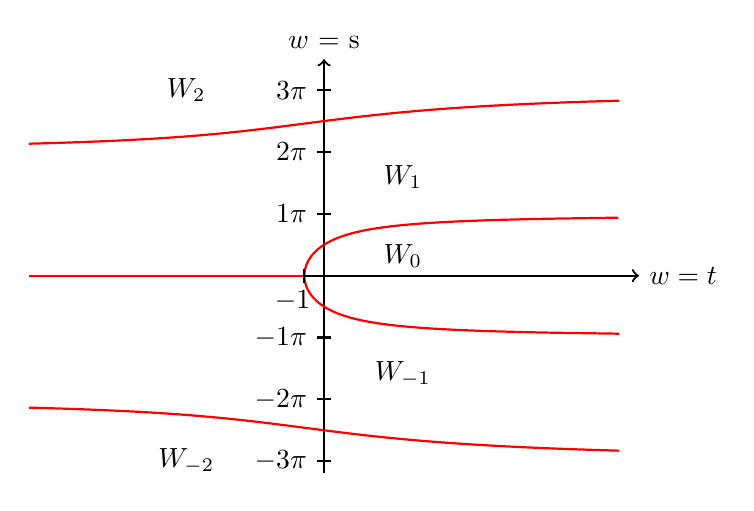
\begin{tikzpicture}[scale = 0.25]
	\def\ticklength{0.35}
	\def\Pi{3.141592653589793}
	\def\ee{2.718281828459045}

	%% Draw w-axes
	\draw[->, thick] (-15, 0) -- (16, 0) node[right] {$\re w = t$};
	\draw[->, thick] (0, -10) -- (0, 11) node[above] {$\im w$ = s};

	%% Draw Branch Curves
	\draw[red,smooth, samples=100, domain=-2.94756:2.94756, variable=\s, thick] 
		plot ({-\s / tan(deg(\s))}, {\s} );
	\draw[red,smooth, samples=200, domain=6.70346:8.88978, variable=\s, thick] 
		plot ({-\s / tan(deg(\s))}, {\s} );
	\draw[red,smooth, samples=200, domain=-8.88978:-6.70346, variable=\s, thick] 
		plot ({-\s / tan(deg(\s))}, {\s} );
	\draw[red, domain=-15:-1, variable=\s, thick] 
		plot ({\s}, 0);

	%% Place Region Labels
	\node (W0) at (4, 1) {$W_0$};
	\node (W-1) at (4, -5) {$W_{-1}$};
	\node (W1) at (4, 5) {$W_{1}$};
	\node (W2) at (-7, {3*\Pi}) {$W_2$};
	\node (W-2) at (-7, {-3*\Pi}) {$W_{-2}$};

	%% Draw im axis tiks
	\foreach \i in {-3, -2, -1, 1, 2, 3} {
		\draw[thick] ({\ticklength}, {\i * \Pi}) -- ({-\ticklength}, {\i * \Pi})
			node[left] {$\i \pi$};
	}

	%% Draw re axis tiks
	\draw[thick] (-1, \ticklength) -- (-1, -\ticklength);
	\node at (-1.6, -\ticklength-0.9) {$-1$};

	\end{tikzpicture}
	\caption{Ranges for the $W_{\pm2}$, $W_{\pm1}$, and $W_0$ branches of the 
		$W$ function.}
	\label{fig:BoundaryCurves}
\end{figure}

Since the map $w \mapsto w e^w$ takes $w = -1$ to $z = -e^{-1}$, 
on pages 17 and 18 in \cite{Corless1996}, 
Corless {\em et al.} proposetaking the branch cut which defines the 
principle branch of $W$ along $\{ z \in \CC ~:~ -\infty < z \leq -e^{-1} \}$, 
and taking all other branch cuts along the entire negative $\re z$-axis.
They further take all branch cuts in such a way that
the branch cuts are closed ``on the top,'' as shown in Figures
\ref{fig:ClosedOnTop} and \ref{fig:OtherBranches}.

\begin{figure}[h!]
	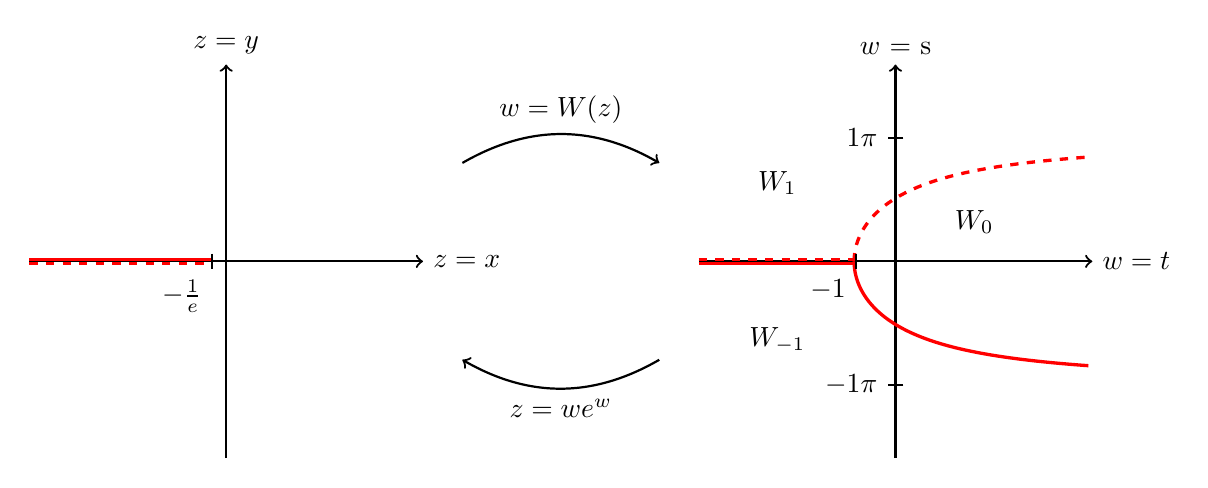
\begin{tikzpicture}[scale=0.5]
		\def\yaxisshift{-4.6}
		\def\ybranchshift{0.05}
		\def\ticklength{0.2}
		\def\Pi{3.141592653589793}
		\def\ee{2.718281828459045}

		%% Draw z-axes
		\draw[->, thick] (-22, 0) -- (-12, 0) node[right] {$\re z = x$};
		\draw[->, thick] (-17, -5) -- (-17, 5) node[above] {$\im z = y$};
		%% Draw w-axes
		\draw[->, thick] (-5, 0) -- (5, 0) 
			node[right] {$\re w = t$};
		\draw[->, thick] (0, -5) -- (0, 5) node[above] {$\im w$ = s};
		%% Draw Map Arrows
		\path[->, thick] (-11, 2.5) edge[bend left] node[auto] {$w = W(z)$} (-6, 2.5);
		\path[->, thick] (-6, -2.5) edge[bend left] node[auto] {$z = w e^w$} (-11, -2.5);

		%% Draw Branch Cut on z-axes
		\draw[very thick, red] 
			(-22, {\ybranchshift}) -- ({-17-1/\ee}, {\ybranchshift});
		\draw[dashed, very thick, red] 
			(-22, {-\ybranchshift}) -- ({-17-1/\ee}, {-\ybranchshift});

		%% Draw Branch Cut along negative Re w axis
		\draw[dashed, very thick, red] (-5, {\ybranchshift}) -- (-1, {\ybranchshift});
		\draw[very thick, red] (-5, {-\ybranchshift}) -- (-1, {-\ybranchshift});

		%% Draw w Branch Curves
		\draw[red,smooth, samples=100, domain=-2.65:-0.001, variable=\s, very thick] 
			plot ({-\s / tan(deg(\s)) -0.05}, {\s} );

		\draw[dashed, red,smooth, samples=100, domain=0.001:2.65, variable=\s, very thick] 
			plot ({-\s / tan(deg(\s)) -0.05}, {\s} );

		%% Label Regions
		\node at (2, 1) {$W_0$};
		\node at (-3, 2) {$W_1$};
		\node at (-3, -2) {$W_{-1}$};

		%% Draw im w tick marks 
		\foreach \i in {-1, 1} {
			\draw[thick] ({\ticklength}, {\i * \Pi}) -- ({-\ticklength}, {\i * \Pi})
				node[left] {$\i \pi$};
		}

		%% Draw re w tick mark
		\draw[thick] (-1, \ticklength) -- (-1, -\ticklength) node[below left] {$-1$};
		% \node at (-1.6, -\ticklength-0.9) {$-1$};


		%% Draw re z tick mark
		\draw[thick] ({-17-1/\ee}, \ticklength) -- ({-17-1/\ee}, -\ticklength) 
			node[below left] {$-\frac{1}{e}$};

	\end{tikzpicture}
	\caption{$W_0$ Branch Cut}
	\label{fig:ClosedOnTop}
\end{figure}



\begin{figure}[h!]
	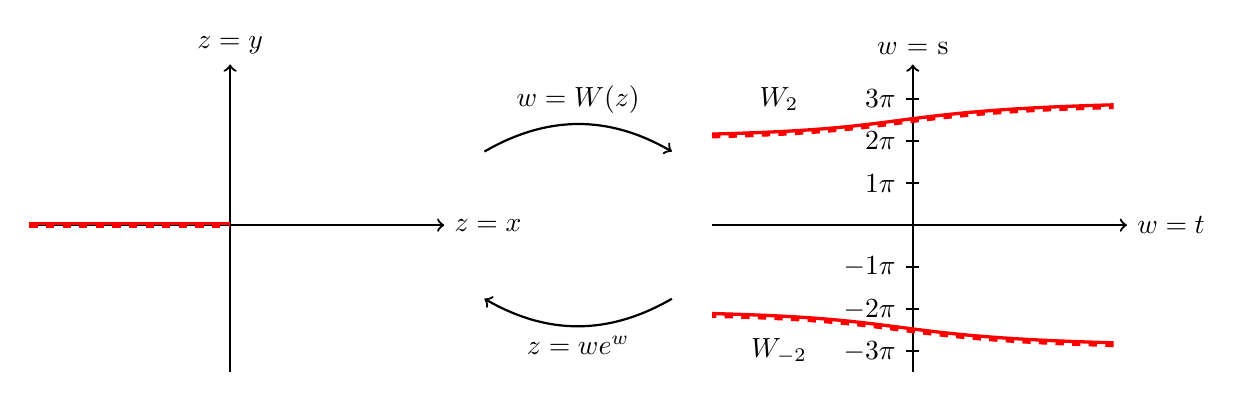
\begin{tikzpicture}[scale=0.17]
		\def\xm{15}
		\def\ashift{1}
		\def\xmin{-\xm}
		\def\xmax{\xm+\ashift}
		\def\ym{11}
		\def\ymin{-\ym}
		\def\ymax{\ym+\ashift}
		\def\yaxisshift{-4.6}
		\def\xshift{51}
		\def\mapshift{3}
		\def\ybranchshift{0.1}
		\def\ticklength{0.5}
		\def\Pi{3.141592653589793}
		\def\ee{2.718281828459045}

		%% Draw z-axes
		\draw[->, thick] (\xmin-\xshift, 0) -- (\xmax-\xshift, 0) 
			node[right] {$\re z = x$};
		\draw[->, thick] (-\xshift, \ymin) -- (-\xshift, \ymax) 
			node[above] {$\im z = y$};

		%% Draw w-axes
		\draw[->, thick] (\xmin, 0) -- (\xmax, 0) node[right] {$\re w = t$};
		\draw[->, thick] (0, \ymin) -- (0, \ymax) node[above] {$\im w$ = s};

		%% Draw Map Arrows
		\path[->, thick] (\xmax-\xshift+\mapshift, \ym/2) edge[bend left] 
			node[auto] {$w = W(z)$} (\xmin - \mapshift, \ym/2);
		\path[->, thick] (\xmin - \mapshift, -\ym/2) edge[bend left] 
			node[auto] {$z = w e^w$} (\xmax-\xshift+\mapshift, -\ym/2);

		%% Draw Branch Cut on z-axes
		\draw[very thick, red] 
			({\xmin-\xshift}, {\ybranchshift}) -- ({0-\xshift}, {\ybranchshift});
		\draw[dashed, very thick, red] 
			({\xmin-\xshift}, {-\ybranchshift}) -- ({0-\xshift}, {-\ybranchshift});

		%% Draw the Branch Curves
		\draw[red,smooth, samples=200, domain=6.70346:8.88978, variable=\s, very thick] 
			plot ({-\s / tan(deg(\s))}, {\s+\ybranchshift} );
		\draw[dashed, red,smooth, samples=200, domain=6.70346:8.88978, variable=\s, very thick] 
			plot ({-\s / tan(deg(\s))}, {\s-\ybranchshift} );
		\draw[red,smooth, samples=200, domain=-8.88978:-6.70346, variable=\s, very thick] 
			plot ({-\s / tan(deg(\s))}, {\s+\ybranchshift} );
		\draw[dashed, red,smooth, samples=200, domain=-8.88978:-6.70346, variable=\s, very thick] 
			plot ({-\s / tan(deg(\s))}, {\s-\ybranchshift} );

		%% Draw im axis tiks
		\foreach \i in {-3, -2, -1, 1, 2, 3} {
			\draw[thick] ({\ticklength}, {\i * \Pi}) -- ({-\ticklength}, {\i * \Pi})
				node[left] {$\i \pi$};
		}

		%% Place Region Labels
		\node (W2) at ({-2*\xm/3}, {3*\Pi}) {$W_2$};
		\node (W-2) at ({-2*\xm/3}, {-3*\Pi}) {$W_{-2}$};

	\end{tikzpicture}
	\caption{$W_k$ ($k \ne 0$) Branch Cuts}
	\label{fig:OtherBranches}
\end{figure}

Corless {\em et al.} further argue in \cite{Corless1996} that each branch
$W_k : \CC \to \ran W_k$ is bijective, which allows us to solve equation
\eqref{eq1:EqnToSolve} and find
\[
	\xi = \frac{1}{2\delta} W_k\big( -2 \delta \zeta(\lambda) \big) + \zeta(\lambda), \qquad k \in \zeta.
\]
Consequently, the only roots of $p(\xi, \lambda)$ which could have a chance of living 
in $\mc R_\delta$ are those corresponding to the $W_{-1}$, $W_0$, and $W_1$ branches.
Now, if $\xi = 0$, then 
\[
	W_k\big( -2 \delta \zeta(\lambda) \big) = -2 \delta \zeta(\lambda).
\]
Since $\zeta$ is a positive, strictly increasing function with $\zeta(0) = 1/(2\delta)$, 
if $\lambda < 0$, then $-1 < -2\delta \zeta(\lambda) < 0$, and if $\lambda \geq 0$, then 
$-2 \delta \zeta(\lambda) \leq -1$. In other words, if $\lambda < 0$ the $\xi = 0$ root of $p$ 
corresponds to the $W_0$ branch, but if $\lambda \geq 0$, then it corresponds to the 
$W_{-1}$ branch. 

On the other hand, if $\xi = \lambda$, then
\[
	W_k\big( -2 \delta \zeta(\lambda) \big) = 2\delta \lambda -2 \delta \zeta(\lambda).
\]
Let $g(\lambda):= 2\delta \lambda -2 \delta \zeta(\lambda)$. 
Note that
\begin{align*}
	\begin{cases}
		0 < \zeta'(\lambda) < \frac{1}{2}, & \text{for } \lambda < 0 \\
		\zeta'(0) = \frac{1}{2}, &  \\
		\frac{1}{2} < \zeta'(\lambda) < 1, & \text{for } \lambda > 0
	\end{cases}
\end{align*}
which implies $g$ is a strictly increasing function. Moreover, since
$\lim_{\lambda\to \infty} g(\lambda) = 0$ and $g(0) = -1$, we see that 
\[
	\begin{cases}
		2\delta \lambda -2 \delta \zeta(\lambda)  < -1, & \lambda < 0 \\
		2\delta \lambda -2 \delta \zeta(\lambda) = -1, & \lambda = 0 \\
		-1 < 2\delta \lambda -2 \delta \zeta(\lambda) < 0, & \lambda > 0
	\end{cases}
\]
Therefore, if $\lambda < 0$ then the $\xi = \lambda$ zero of $p$ corresponds to the 
$W_{-1}$ branch, but if $\lambda \geq 0$, it corresponds to the $W_{0}$. Moreover, 
given that $-2\delta \zeta(\lambda)$ lies on the negative real axis and hence on the branch
cut used for $W_k$, $k \ne 0$, each value of 
$2\delta\xi-2\delta\zeta(\lambda) = W_k\big(-2\delta\zeta(\lambda)\big)$ ($k \ne 0$) lies on the boundary
between the respective ranges of the $W$ branches. In particular, given that 
the strip $\big\{ z ~:~ -2\pi \leq \im z \leq 2 \pi \big\}$ does not contain
any part of the boundary between $\ran W_{-2}$ and $\ran W_{-1}$ or any part 
of the boundary between $\ran W_1$ and $\ran W_2$, this strip contains exactly 
two values of $W\big(-2 \delta \zeta(\lambda) \big)$. Since
\[
	\mc R_\delta = \frac{1}{2\delta}\big\{ z ~:~ -2\pi \leq \im z \leq 2 \pi \big\}+\zeta(\lambda),
\]
the strip $\mc R\delta$ contains exactly two roots of $p$\textemdash{}precisely as claimed.


\end{document}